% Capitolo 1 - Introduzione
\refsection
\chapter{Introduzione}
\label{cap1_introduction}

\section{Contesto e Motivazione della Ricerca}

\subsection{La Complessità Sistemica della Grande Distribuzione Organizzata}

Il settore della Grande Distribuzione Organizzata (GDO) in Italia gestisce un'infrastruttura tecnologica la cui complessità è paragonabile a quella di operatori di telecomunicazioni o servizi finanziari. Con 27.432 punti vendita attivi\autocite{istat2024}, 45 milioni di transazioni elettroniche giornaliere e requisiti di disponibilità superiori al 99.9\%, la GDO rappresenta un caso di studio unico per l'ingegneria dei sistemi distribuiti \textit{mission-critical}.

L'infrastruttura IT della GDO moderna deve garantire simultaneamente continuità operativa H24 in ambienti fisicamente distribuiti, processare volumi transazionali con picchi del 300-500\% durante eventi promozionali\autocite{Osservatorio2024}, proteggere dati sensibili di pagamento e personali sotto multiple normative, integrare sistemi legacy con tecnologie cloud-native, e gestire la convergenza tra Information Technology (IT) e Operational Technology (OT). Ogni punto vendita, infatti, non è solo un terminale commerciale ma un nodo computazionale autonomo che deve mantenere sincronizzazione con i sistemi centrali, garantire operatività anche in caso di disconnessione temporanea e rispettare stringenti requisiti di sicurezza e compliance. Questa architettura distribuita crea sfide uniche in termini di gestione della consistenza dei dati, propagazione degli aggiornamenti e contenimento delle minacce informatiche.

\subsection{L'Evoluzione del Panorama Tecnologico e delle Minacce}

Il settore sta attraversando una trasformazione profonda, guidata da tre forze convergenti: 
\begin{itemize}
	\item La prima è \textbf{la trasformazione infrastrutturale}: il 67\% delle organizzazioni GDO europee ha iniziato processi di migrazione da data center tradizionali verso modelli cloud-ibridi\autocite{gartner2024cloud}, una transizione che richiede un ripensamento fondamentale dei modelli operativi e di sicurezza.
	\item La seconda è \textbf{l'evoluzione delle minacce informatiche}: l'incremento del 312\% negli attacchi ai sistemi retail tra il 2021 e il 2023\autocite{enisa2024retail} e l'emergere di attacchi cyber-fisici (es. compromissione di sistemi di refrigerazione \textbf{HVAC - Heating, Ventilation, and Air Conditioning)} impongono un radicale cambio di strategia difensiva. 
	\item La terza forza è \textbf{la crescente complessità normativa}: l'entrata in vigore simultanea del \textbf{Payment Card Industry Data Security Standard (PCI-DSS) v4.0}, gli aggiornamenti del \textbf{General Data Protection Regulation (GDPR)} e l'implementazione della \textbf{Direttiva Network and Information Security 2 (NIS2)} creano un panorama che, se affrontato con metodi tradizionali, può costare fino al 2-3\% del fatturato \autocite{ponemon2024compliance}.
\end{itemize}

\section{Problema di Ricerca e Gap Scientifico}

L'analisi della letteratura scientifica e tecnica rivela una significativa disconnessione tra la ricerca accademica e le necessità pratiche del settore GDO. Questo gap rappresenta l'opportunità per un contributo originale e si manifesta in tre aree principali:
\begin{itemize}
    \item \textbf{Mancanza di approcci olistici:} Gli studi esistenti tendono a trattare separatamente l'infrastruttura, la sicurezza cloud e la compliance normativa, ignorando le complesse interdipendenze sistemiche che caratterizzano gli ambienti reali della GDO.
    \item \textbf{Assenza di modelli economici validati:} La letteratura accademica manca di modelli di TCO (Total Cost of Ownership) e ROI (Return on Investment) specificamente calibrati per il settore retail e validati empiricamente, strumenti indispensabili per giustificare le decisioni architetturali al management.
    \item \textbf{Limitata considerazione dei vincoli operativi:} Le ricerche su paradigmi come Zero Trust o cloud migration sono spesso sviluppate in contesti generici e non considerano vincoli critici della GDO quali la continuità H24, la gestione di personale con limitate competenze tecniche o la necessità di performance transazionali estreme.
\end{itemize}
Manca un approccio integrato che consideri le interdipendenze sistemiche tra questi elementi e fornisca un framework operativo unificato. Alla luce di ciò, il problema di ricerca principale può essere formulato come segue:

\textbf{Come progettare e implementare un'infrastruttura IT per la Grande Distribuzione Organizzata che bilanci in maniera ottimale sicurezza, performance, compliance e sostenibilità economica nel contesto di evoluzione tecnologica accelerata e minacce emergenti?}

\section{Obiettivi e Contributi Originali Attesi}
\subsection{Obiettivo Generale}
L'obiettivo generale di questa ricerca è sviluppare e validare un framework integrato, denominato \textbf{GIST (GDO Integrated Security Transformation)}, per la progettazione e gestione di infrastrutture IT sicure nella GDO. Tale framework deve considerare l'intero stack tecnologico, dall'infrastruttura fisica alle applicazioni cloud-native, fornendo un approccio sistemico che sia rigoroso, ripetibile e flessibile.

\subsection{Obiettivi Specifici e Misurabili}
Per raggiungere l'obiettivo generale, la ricerca persegue quattro obiettivi specifici e misurabili:
\begin{itemize}
    \item \textbf{(OS1)} Analizzare l'evoluzione delle minacce e l'efficacia delle contromisure, mirando a documentare una riduzione degli incidenti superiore al 40\%.
    \item \textbf{(OS2)} Modellare l'impatto delle architetture cloud-ibride su performance e costi, sviluppando un modello predittivo con un coefficiente di determinazione R² superiore a 0.85.
    \item \textbf{(OS3)} Quantificare i benefici di un approccio compliance-by-design, dimostrando una riduzione dei costi di conformità superiore al 30\%.
    \item \textbf{(OS4)} Sviluppare linee guida pratiche per la trasformazione, validate per garantirne l'applicabilità ad almeno l'80\% delle organizzazioni target.
\end{itemize}

\subsection{Contributi Originali Attesi}
Il perseguimento di tali obiettivi porterà allo sviluppo di contributi originali sia per la teoria che per la pratica:
\begin{enumerate}
    \item \textbf{Framework GIST:} Un modello olistico e multi-livello per la valutazione e progettazione di infrastrutture sicure nella GDO.
    \item \textbf{Modello Economico GDO-Cloud:} Un framework quantitativo per l'analisi di TCO e ROI, validato empiricamente e specifico per il settore.
    \item \textbf{Matrice di Integrazione Normativa:} Una mappatura sistematica delle sinergie tra PCI-DSS 4.0, GDPR e NIS2 per un'implementazione unificata.
    \item \textbf{Framework Digital Twin GDO-Bench:} Un ambiente di simulazione per la generazione di dataset sintetici realistici, che costituirà una base metodologica per future ricerche.
\end{enumerate}

\section{Ipotesi di Ricerca}
La ricerca si propone di validare le seguenti tre ipotesi, formulate per essere empiricamente testabili attraverso il framework Digital Twin.
\begin{itemize}
    \item \textbf{H1 (Evoluzione Architetturale):} L'implementazione di architetture cloud-ibride, progettate secondo pattern specifici per la GDO, permette di conseguire e mantenere livelli di disponibilità del servizio \textbf{(SLA - Service Level Agreement)} superiori al 99.95\% in presenza di carichi transazionali variabili, ottenendo come beneficio aggiuntivo una riduzione del TCO superiore al 30\% rispetto ad architetture tradizionali on-premise.
    \item \textbf{H2 (Sicurezza):} L'integrazione di principi Zero Trust in architetture GDO distribuite riduce la superficie di attacco aggregata di almeno il 35\%, mantenendo l'impatto sulla latenza delle transazioni critiche entro 50 millisecondi.
    \item \textbf{H3 (Compliance):} L'implementazione di un sistema di gestione della compliance basato su principi di compliance-by-design e automazione permette di soddisfare simultaneamente i requisiti di PCI-DSS 4.0, GDPR e NIS2 con un overhead operativo inferiore al 10\% delle risorse IT, conseguendo una riduzione dei costi totali di conformità del 30-40\%.
\end{itemize}

\section{Metodologia della Ricerca}
Per validare le ipotesi formulate, la ricerca adotta un \textbf{approccio \textit{mixed-methods}} che unisce il rigore della simulazione quantitativa con approfondimenti qualitativi derivanti da best practice di settore.

Data la sensibilità commerciale e i vincoli di riservatezza che impediscono l'accesso a dati operativi reali su larga scala, il nucleo della validazione quantitativa si affida al \textbf{framework Digital Twin GDO-Bench}, uno dei contributi originali di questa tesi. Questo ambiente di simulazione genera dataset sintetici ma \textbf{statisticamente realistici}, replicando le dinamiche di una rete GDO complessa. Il Digital Twin è stato \textbf{calibrato utilizzando dati aggregati pubblici, report di settore (ENISA, Gartner) e parametri tecnici documentati}, assicurando che i pattern transazionali, il traffico di rete e la distribuzione degli eventi di sicurezza siano rappresentativi del contesto reale italiano.

All'interno di questo ambiente simulato, verrà condotta un'analisi sistematica per testare le ipotesi, eseguendo \textbf{simulazioni Monte Carlo} per valutare l'impatto di diverse architetture (H1), configurazioni di sicurezza (H2) e controlli di compliance (H3) su un ampio spettro di scenari operativi. Le metriche generate (log da sistemi \textbf{SIEM}, indicatori di performance, stime di costi \textbf{CAPEX/OPEX}) saranno analizzate statisticamente. Questo approccio garantisce la \textbf{testabilità empirica delle ipotesi in un ambiente controllato, ripetibile e scientificamente valido}.

\section{Delimitazioni e Limitazioni della Ricerca}

\subsection{Delimitazioni (Scope)}
La ricerca si focalizza specificamente su organizzazioni GDO italiane con 50-500 punti vendita e un fatturato annuo compreso tra 100 milioni e 2 miliardi di euro, considerando il periodo 2022-2024. Sono deliberatamente esclusi operatori di e-commerce puro, micro-retail, settori non-food e mercati extra-europei.

\subsection{Limitazioni}
La ricerca riconosce che la validazione basata su simulazione, pur essendo metodologicamente robusta, potrebbe non catturare tutte le sfumature delle implementazioni reali. I risultati sono primariamente applicabili al contesto italiano ed europeo e l'orizzonte temporale potrebbe non cogliere tutti i benefici a lungo termine.

\section{Rilevanza della Ricerca}
\subsection{Rilevanza Accademica}
La ricerca contribuisce all'avanzamento delle conoscenze nei domini dei sistemi distribuiti mission-critical, della sicurezza informatica in contesti operativi complessi e dell'ingegneria economica dei sistemi IT, proponendo modelli innovativi e specifici per il settore.

\subsection{Rilevanza Pratica e Sociale}
L'impatto pratico si manifesta nel supporto alle decisioni di investimento, nella riduzione dei rischi nei progetti di trasformazione e nell'ottimizzazione dei costi di compliance. A livello sociale, il lavoro contribuisce alla protezione dei dati di milioni di consumatori e alla resilienza di infrastrutture critiche per l'approvvigionamento alimentare nazionale.

\section{Struttura della Tesi}
La tesi si articola in cinque capitoli che guidano il lettore dalla definizione del problema alla presentazione di una soluzione validata, come illustrato nella Figura \ref{fig:thesis_structure}.

\begin{figure}[htbp]
\centering
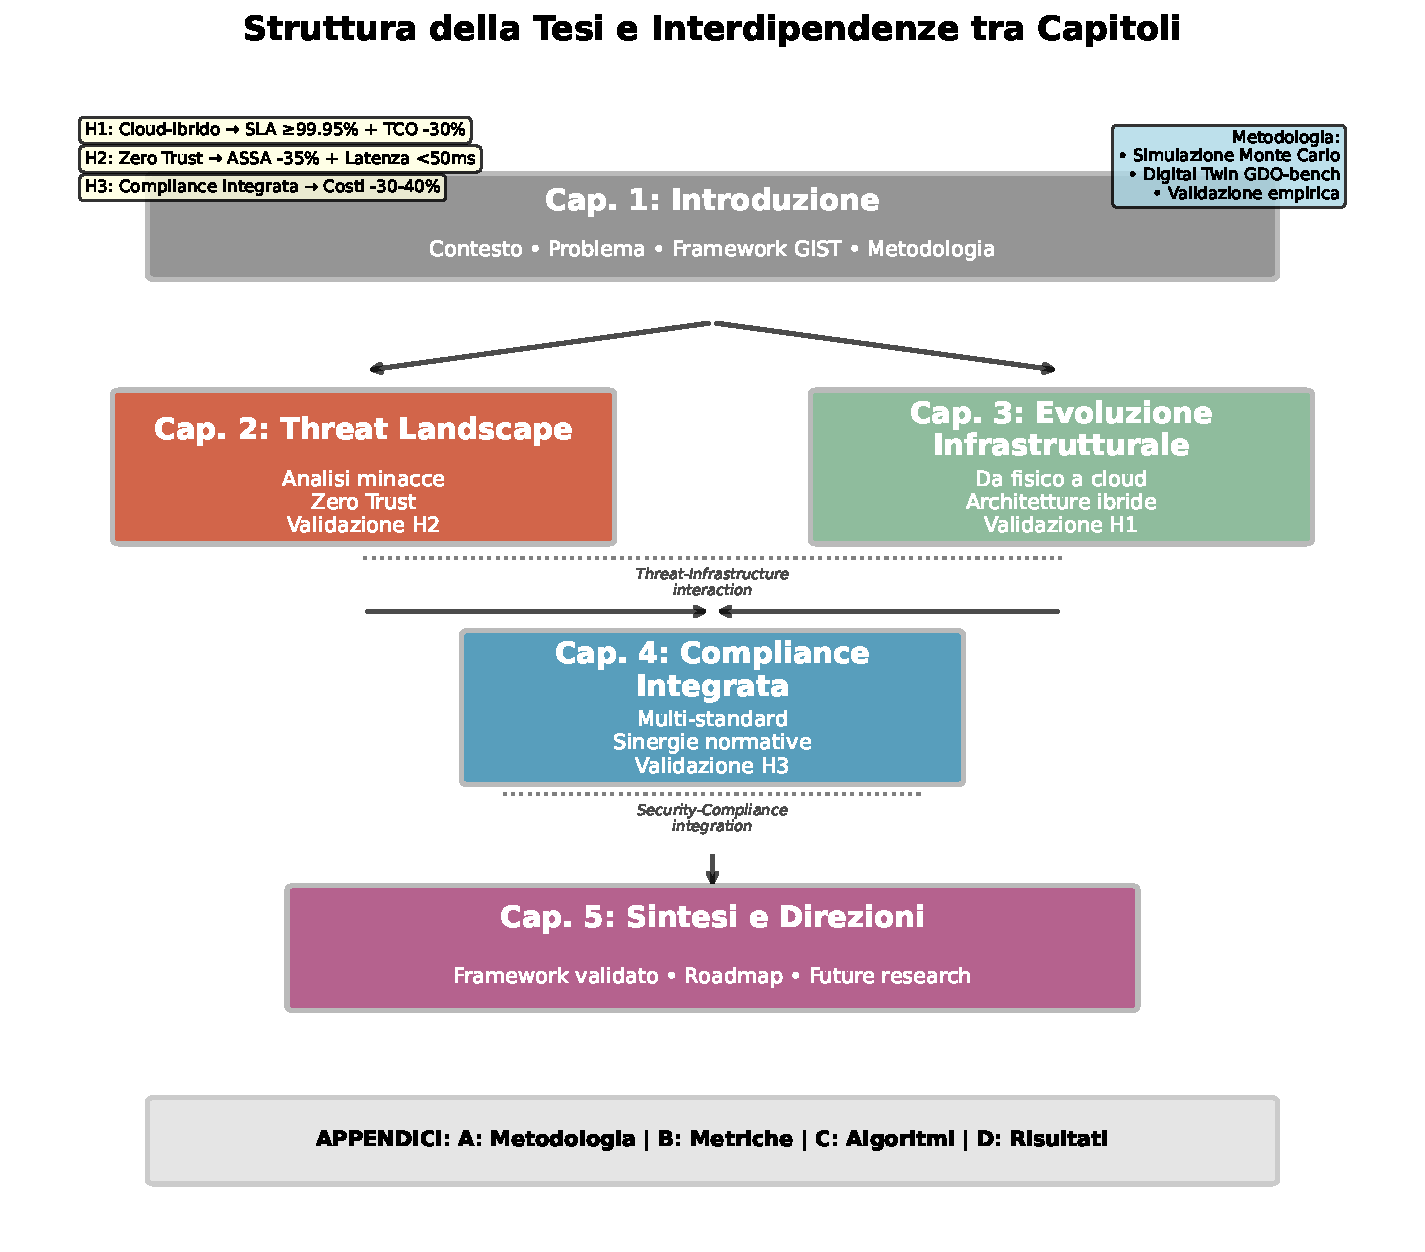
\includegraphics[width=1\textwidth]{thesis_figures/cap1/fig_1_4_thesis_structure.pdf}
\caption{Struttura della tesi e interdipendenze tra capitoli. Il diagramma mostra il flusso logico dalla definizione del problema (Capitolo 1) attraverso l'analisi delle componenti specifiche (Capitoli 2-4) fino alla sintesi e validazione del framework completo (Capitolo 5).}
\label{fig:thesis_structure}
\end{figure}

Il Capitolo 2 analizza il panorama delle minacce, il Capitolo 3 esamina l'evoluzione infrastrutturale verso il cloud-ibrido, il Capitolo 4 affronta la compliance integrata e la governance. Infine, il Capitolo 5 sintetizza i risultati, presenta il framework GIST validato e delinea le direzioni strategiche future.

\clearpage
\printbibliography[
    heading=subbibliography,
    title={Riferimenti Bibliografici del Capitolo 1},
]

\endrefsection
